\chapter{Graphene.js: Building Reusuable Web Components for Data Visualization}

\section{Purpose}

The purpose of this chapter is to introduce Graphene.js \autocite{gu2014graphene}, a framework for creating data-driven visualizations and user interfaces.
In addition, the Graphene.js approach to data visualization is contrasted to currently established JavaScript drawing libraries.
Graphene is the key component of the user interface for all other applications described in this body of work.

\section{Motivation}

Graphical representations of information are valuable for presenting complex information quickly and clearly. \autocite{newsom2007public, smiciklas2012power}
They can vastly improve comprehension by using graphics to enhance the human visual system’s ability to see patterns and trends. \autocite{heer2010tour, sears2007human}
Meanwhile, the Internet and World Wide Web \autocite{berners2000weaving} has become perhaps the most powerful medium for information sharing. \autocite{bollacker1998citeseer, wilkinson2003motivations, page1999pagerank}
Modern web applications have many advantages over traditional desktop applications.
Software developers typically face a challenge in deploying software applications to their clients (Figure~\ref{fig:deployment-problem}).
End users may use a wide variety of platforms, such as Apple OS X, Microsoft Windows, and Linux for desktop computers and Apple iOS, Google Android, and Microsoft Windows Phone for mobile devices.
Each platform has a different pattern for building native binaries, which requires special expertise and is an obstacle particularly for smaller development teams and research labs.
Web applications are inherently cross platform, available on all devices with a capable web browser (Figure~\ref{web-app-deployment}).
Updates are also delivered immediately, which is typically not the case for desktop softwares.
Thus, HTML5 web applications are a compelling platform for biomodeling applications as well.

\begin{figure}
  \centering
  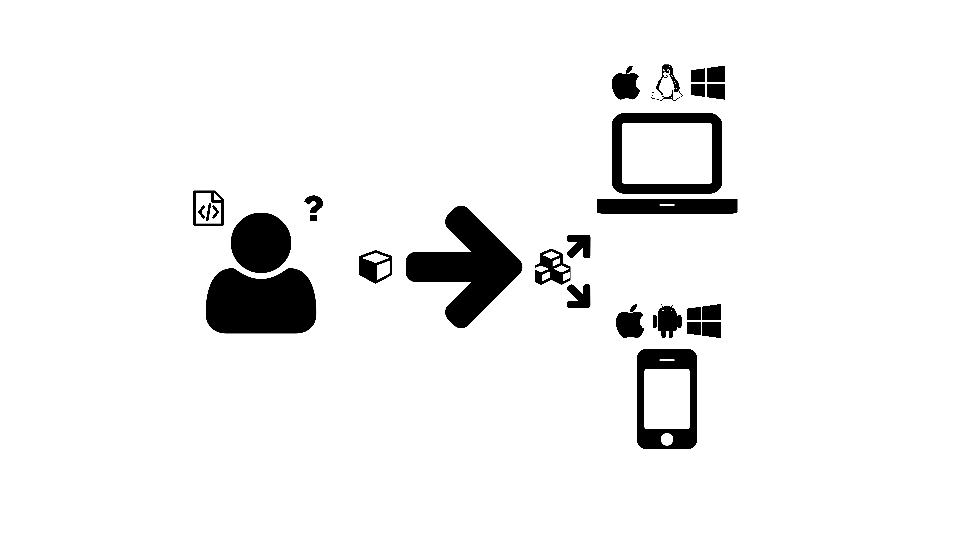
\includegraphics[width=\textwidth,natwidth=610,natheight=642]{images/deployment-problem.png}
  \caption{Software developers often face a challenge in deploying their code base to end users due to the widespread use of multiple platforms.}
  \label{fig:deployment-problem}
\end{figure}
\begin{figure}
  \centering
  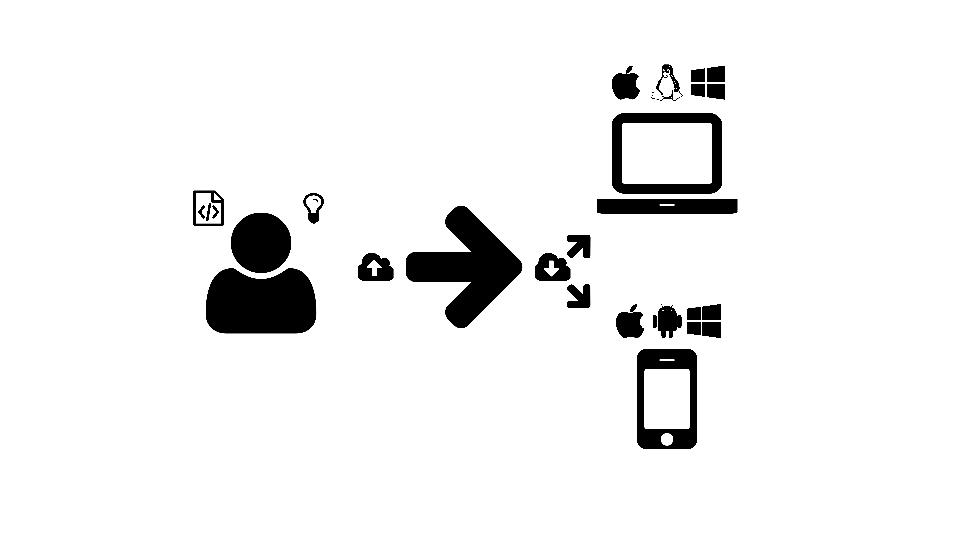
\includegraphics[width=\textwidth,natwidth=610,natheight=642]{images/web-app-deployment.png}
  \caption{Web applications solve the cross-platform problem.}
  \label{fig:web-app-deployment}
\end{figure}

\subsection{Few systems biology software packages are built using HTML5 web technologies}
Modeling standards and open source software packages, as reviewed in  Software in chapter~\ref{chap:background}, have been a boon to the biomedical research community.
While there are a wide variety of powerful tools that have been developed over the years, there is a distinct lack of web applications.
One way to get a sense of the current landscape of modeling software is to consider the SBML Software Guide \autocite{sbml2014software}, which has conveniently organized and characterized publicized SBML compatible software.
Of the 96 closed-source software packages listed in the Software Guide, only 24 contain any type of web based features and only one can be considered an HTML5 web application \autocite{olivier2004web}.
Of the 166 free and open source softwares listed, just 37 contain any web capabilities, and none of which are an HTML5 application.
\subsection{Systems biology software is complex and building complex web applications is difficult}
There are several obstacles to building biomodeling web applications, which may explain the absence of web applications in the biomodeling domain.
Scientific libraries that most biomodeling software depends on have been intended for desktop use, which can also be used server-side in a web application, but requires additional expertise.
Furthermore, designing and implementing complex graphical user interfaces (GUIs) on the web is a nontrivial engineering challenge.
As discussed in section~\ref{sec:html5} HTML was originally designed as a markup language for communicating static pages that contain text and limited amounts of media, while using CSS for styling.
The rise of JavaScript support within browsers allowed web pages to evolve more interactive behaviors, leading eventually to the web applications of today.
However, JavaScript was originally intended for simple scripts which manipulate the DOM, and this legacy has lead to challenges in scaling increasingly complex JavaScript applications.

\subsubsection{JavaScript code bases that treat the DOM as data model are difficult to scale}

\begin{figure}
  \centering
  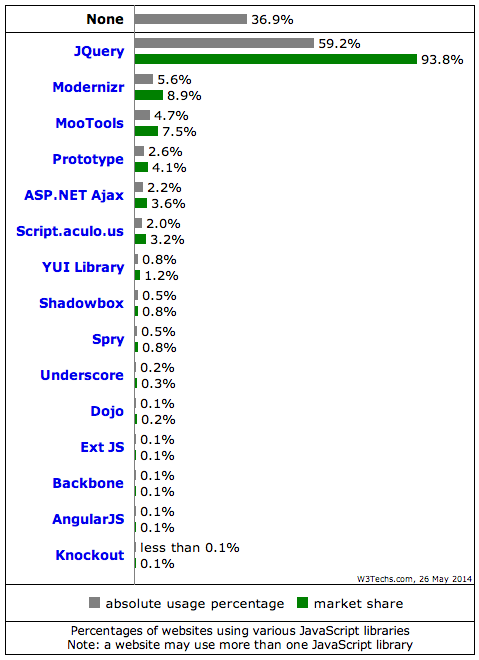
\includegraphics[width=\textwidth,natwidth=610,natheight=642]{images/jquery-marketshare.png}
  \caption{Market share client-side JavaScript libraries as of May 2014. \autocite{w3techs2014javascript}}
  \label{fig:jquery-marketshare}
\end{figure}

By far, the most popular client-side JavaScript library is jQuery. \autocite{w3techs2014javascript}
Of the 59.2\% of websites that contain JavaScript, JQuery is present in 93.8\% of them (Figure~\ref{fig:jquery-marketshare}).
In web applications that primarily rely on JQuery, the most common design pattern is to treat the DOM as the data model (DOMAM).
In DOMAM, controller logic acts on the DOM directly, creating, updating, and deleting DOM components when the application data model changes.
DOMAM style applications are easy to implement for small applications, but as they grow larger and more complex, the lack of separating the model and view leads to difficulties for software maintenance and continued development.
Section~\ref{sec:declarative-vs-imperative} provides more description and examples on the weaknesses of the DOMAM pattern, as it is perhaps easier to understand when compared to the alternative solution.

\subsection{Most existing drawing libraries follow the jQuery DOM manipulation pattern and are less suited for complex and customizable visualizations}
A key component of GUI for computational systems biology application is in its bio-network graph layout.
In order to reduce duplication of code effort and promote programming best practices, it is desirable to use a software library when solving recurring software problems.
However, most JavaScript drawing libraries encourage the DOMAM pattern or lack customization options.
Being able to customize the visual layout allows for greater design control of an application's UI. 
Better web designs are important because it may increase user engagement and likelihood of revisiting. \autocite{rosen2004website}


\section{Solution}

\subsection{Graphene.js allows for easily customizable and reusuable web diagrams}
Graphene.js addresses these issues by using a different approach.
Graphene creates interactive diagrams through two-way-binding of the application data model to a customizable SVG template.
Thus, no custom rendering engine is required as it is performed by the browser, and the rich SVG vocabulary (which may be created through a text editor or through a graphical SVG drawing program) may be used to define nearly any type of edge, arrow marker, or Bezier curve.
Graphene templates may also be customized for visualizations beyond node-edge graphs, such as charts and animations.


Cytoscape.js \autocite{cytoscape2014js} is a graph drawing library and a potential choice for network visualization. 
It contains an impressive HTML5 Canvas based rendering engine, but currently lacks the ability to customize the following:

\begin{itemize}
\item Color gradients for nodes
\item Marker ends and node shapes beyond a predefined set
\item Control points for Bezier curves
\item Placement of edge start and end points
\end{itemize}

In addition, since Cytoscape.js produces a canvas drawing and not DOM elements, the graph elements are unable to be used with other JavaScript libraries (for example a popover plugin that acts on each node) nor bound to custom events.
Cytoscape Web \autocite{cytoscape2014web} is a similar library, but is based on Adobe Flash, which limits its utility for cross platform deployment.

\subsection{Declarative vs. Imperative: Data-binding over DOM manipulation}
\label{sec:declarative-vs-imperative}

Graphene uses Angular.js \autocite{google2014angular} to provide a Model-View-Controller \autocite{krasner1988description} interface for implementing layouts.
Here we will discuss the differences between the DOMAM/jQuery pattern and Angular MVC approach, which will help explain the design decisions behind Graphene.
Consider this jQuery example of fetching JSON data from an endpoing:

\begin{lstlisting}[language=JavaScript]
$.ajax({
  url: '/myData.json',
  success: function(data, status) {
    $('ul#log').append('<li>Data Received!</li>');
  }
});
\end{lstlisting}

\texttt{\$.ajax} something something darkside

\begin{lstlisting}[language=html]
<ul class="messages" id="log">
</ul>
\end{lstlisting}

\begin{lstlisting}[language=JavaScript]
$http( '/myEndpoint.json' ).then( function ( response ) {
  $scope.log.push( { msg: 'Data Received!' } );
});
\end{lstlisting}

\begin{lstlisting}[language=html]
<ul class="messages">
  <li ng-repeat="entry in log">{{ entry.msg }}</li>
</ul>
\end{lstlisting}

\begin{lstlisting}[language=html]
<div class="messages">
  <div class="alert" ng-repeat="entry in log">
    {{ entry.msg }}
  </div>
</div>
\end{lstlisting}

Raphael.js \autocite{sencha2014raphael}








\section{Implementation}
\subsection{Angular.js is used for data-binding}
\subsection{D3.js is used for SVG manipulation}
\subsection{Yeoman build chain allows for easy integration}

\section{Future Directions}
\autocite{w3c2014components}
\autocite{w3c2014templating}
\autocite{polymer2014templating}
